\documentclass[12pt]{amsart}
\usepackage[margin=1in]{geometry}                % See geometry.pdf to learn the layout options. There are lots.
\geometry{letterpaper}                   % ... or a4paper or a5paper or ... 
%\geometry{landscape}                % Activate for for rotated page geometry
\usepackage[parfill]{parskip}    % Activate to begin paragraphs with an empty line rather than an indent
\usepackage{graphicx}
\usepackage{amssymb}
\usepackage{epstopdf}
\DeclareGraphicsRule{.tif}{png}{.png}{`convert #1 `dirname #1`/`basename #1 .tif`.png}

\title{Logistic Regression}
%\author{The Author}
\date{\today}                                           % Activate to display a given date or no date

\begin{document}
\maketitle

\section{Probabilities and Odds}

\subsection{Probabilities}

Odds are related to probabilities so let's refresh ourselves on probabilities. The probability gives the proportion of time something is expected to happen, when the basic process is done over and over again, independently and under the same conditions\footnote{Pg. 222 in Freedman, Pisani, and Purves}. Often, probabilities are thought of in terms of success or failure. Let N be the number of times an event is expected to happen when repeating a process over and over again. Let M be the number of times the process was repeated:

\[ \text{Probability of success: } p = \frac{N}{M} \]

You can find the probability of something not happening by subtracting $p$ from 1:

\[ \text{Probability of failure: } q = 1-p \]

Another way to think about it is: the probability of an event given a process is the total possible process outcomes that include the event (N) divided by the total possible process outcomes (M).

Consider the simple case of flipping a coin. You find the probability of getting heads by dividing the number of possible ways to get heads (one) by the total possibilities (two - heads or tails). So the probability is $\frac{1}{2} = 0.5$.

Consider a less simple example of drawing cards. The probability of drawing an ace from a fair 52 card deck would be the number of aces in the deck (four) divided by the total number of cards (52) so the probability is $\frac{4}{52} = 0.077$.

Consider a class of 20 people. 15 of the students are female identified. 5 are male identified. What is the probability of randomly picking a female identified student if I randomly pick just one student? We divide the number of female identified students (total possible ways I can pick a female identified student) by the number of students (total possible ways I could pick any student): $\frac{15}{20} = 0.75$

\subsection{Odds}

Odds are related to probabilities, but are different. Odds are calculated by dividing the probability of success by the probability of failure. Another way to think about: let N be the number of times an event is expected to happen when repeating a process over and over again and M be the number of times you repeated the process:

\[ \text{Odds: } O = \frac{N}{M-N} = \frac{p}{1-p} \]

So revisiting the flipped coin, the odds of getting heads would be equal to the probability of getting heads divided by the probability of getting tails (not-heads):

\[ \frac{0.5}{0.5} = 1.0 \]

So if you have a fifty percent chance (or probability) of something happening, then the odds of it happening is 1. The odds of drawing an ace from a deck of cards can be calculated a couple different ways. First, we could divide the probability we calculated above by the 1 minus the probability:

\[ \frac{0.077}{1-0.077} = 0.083 \]

Or we can divide the number of aces in the deck by the number of not aces in the deck:

\[ \frac{4}{52-4} = 0.083 \]

For the classroom example, we have both possible ways to calculate the odds again. Divide the probability of picking a female identified student by the probability of not picking a female identified student. Or divide the number of female identified students by the number of not female identified students.

\[ \frac{0.75}{1-0.75} = 3.0 \]

\[ \frac{15}{5} = 3.0 \]

Notice that if there is less than a 50\% chance of something happening, the odds will be less than one. If there is a greater than 50\% chance of something happening, the odds will be greater than one.

\newpage

\subsection{Odds Ratios}

Finally, we can compare the odds of two events happening by calculating their odds ratio. Odds ratios are calculated by dividing the odds of one event by the odds of another event.

Consider a large Sociology program with the following stats:

\begin{table}[htb]
\caption{Sociology Admissions\label{tab:admin}}
\begin{tabular}{l c c}
\hline
& Men & Women\\ \hline
Applied & 150 & 200\\
Admitted & 20 & 15\\
\hline
\end{tabular}
\end{table}

\textbf{What is the probability of a man being admitted? A woman?}

The probability of a man being admitted is the number of men admitted divided by the number that have applied:

\[ p = \frac{20}{150} = 0.133 \]

For women, we do the same thing:

\[ p = \frac{15}{200} = 0.075 \]

So men have a higher chance of getting in than women.

\textbf{What is the odds of admission for men and women?}

Odds are found by dividing the probability of success by the probability of failure:

\[ \text{men: } O = \frac{20}{150-20} = \frac{0.133}{1-0.133} = 0.154 \]

\[ \text{women: } O = \frac{15}{200-15} = \frac{0.075}{1-0.075} =  0.081 \]

Again, men have higher odds of being admitted than women.

\textbf{What is the odds ratio of men to women?}

The odds ratio is found by dividing the odds of one event by the odds of another event. So the odds ratio for admission would be the odds of men divided by the odds of women:

\[ OR = \frac{0.154}{0.081} = 1.9 \]

So men have about twice the odds of being admitted than women do. This is an odds ratio.

Odds ratios, then, are a way to describe the relative likelihood of two events happening. 

\section{Logistic Regression}


So far we've learned how to do regression analysis when our dependent variable is a continuous variable. What do we do when we have a dichotomous dependent variable? Well, we could still use OLS. Doing so gives us a linear probability model - the coefficients are interpreted as the effect of the independent variable on the probability of the dependent variable being 1. Unfortunately, using OLS regression on a dichotomous variable results in some major violations of the assumptions of OLS, most egregious of which is the normality assumption of the residuals. Additionally, OLS doesn't know that probabilities can only be between zero and one, so on the low and high ends of your data, OLS can predict probabilities that are less than zero or greater than one. Linear probability models like these are a good starting point when analyzing data, but should not be what you ultimately use. Instead, we can use logistic regression.

\subsection{The Logistic Curve}

Logistic regression is used when your dependent variable is dichotomous and models the odds of something happening. 

Remember that the odds of something happening is the probability that it will happen divided by the probability that it will not happen:

\[ \text{Odds} = \frac{p}{1-p} \]

Logistic regression models the log odds of the dependent variable with a linear combination of independent variables:

\[ \log \left( \frac{p}{1-p} \right) = \alpha + \beta_1 x_1 ...\]

Because the left side of the equation is $\log(\frac{p}{1-p})$ and not simply $y$ or $\log(y)$, the right side of the equation gets fitted to a logistic curve instead of  a straight line. Figure \ref{fig:one} shows the logistic curve. Notice that the curve is bounded between 0 and 1, which is appropriate for our dichotomous dependent variable.

\begin{figure}[htb]
\caption{Logistic Curve\label{fig:one}}
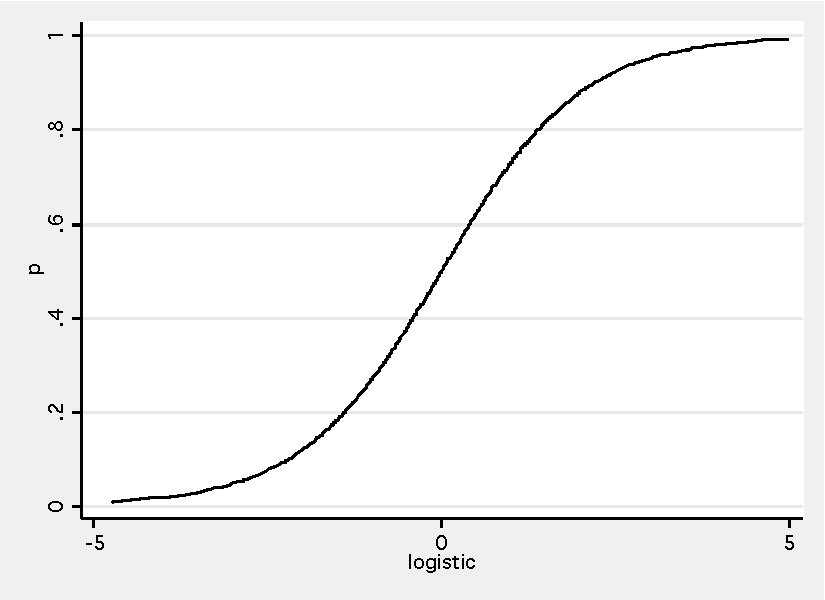
\includegraphics[width=0.8\textwidth]{logisticcurve}
\end{figure}

\subsection{Logistic Regression}

Let's see logistic regression in action. Using the \texttt{hire771} dataset, we'll run some logistic regressions on whether or not someone is assigned to the home office. Logistic regression in STATA requires our dependent variable to be coded 0 and 1 only, so we need to transform the \texttt{homeoff} variable:

\texttt{gen HO = homeoff == 1}

Then we run our regression. In STATA, we use the \texttt{logit} command. We specify the model exactly the same as we did with \texttt{regress}. Figure \ref{fig:two} has the STATA output from the logit command.

\begin{figure}[htb]
\caption{Logit output\label{fig:two}}
\begin{verbatim}
. logit HO sex

Iteration 0:   log likelihood = -1404.5207
Iteration 1:   log likelihood = -1325.0842
Iteration 2:   log likelihood = -1310.9342
Iteration 3:   log likelihood = -1310.9328

Logistic regression                               Number of obs   =       3131
                                                  LR chi2(1)      =     187.18
                                                  Prob > chi2     =     0.0000
Log likelihood = -1310.9328                       Pseudo R2       =     0.0666

------------------------------------------------------------------------------
          HO |      Coef.   Std. Err.      z    P>|z|     [95% Conf. Interval]
-------------+----------------------------------------------------------------
         sex |  -1.559599   .1101681   -14.16   0.000    -1.775524   -1.343673
       _cons |  -.4071907   .0928957    -4.38   0.000     -.589263   -.2251184
------------------------------------------------------------------------------
\end{verbatim}
\end{figure}

Let's quickly explore this output. First, notice that instead of an ANOVA table, we get iterations of log likelihoods. Logistic regression uses maximum likelihood methods to calculate the coefficients of the model because there is no arithmetic methods of calculating the coefficients directly. Instead, STATA runs through several iterations of guesses until it finds one that maximizes the likelihood parameter\footnote{See Prof. Noymer's handout on maximum likelihood for a more in depth explanation}. 

Second, we get a $\chi^2$ test instead of a F test. This tests for the same thing, though - is the current model better at explaining the data over the null model? We also get a pseudo-$R^2$. Since we don't have an ANOVA table, we don't have a real $R^2$ statistic. The pseudo-$R^2$ is an approximation of the $R^2$ statistic and can be interpreted the same way - how well the model fits the data.

The important part of the output is the table containing our coefficients. We see a sex coefficient as well as our \texttt{\_cons} term just like in OLS regression. However, the coefficients are interpreted slightly differently. In this case, the sex coefficient gives the effect of being a woman on the log odds of being assigned to the home office. Now, log odds doesn't mean much substantively, but we can tell a couple things from the coefficient. First, the coefficient is negative so we know that being a woman decreases the odds of being assigned to the home office. Second, the coefficient is pretty large, so the effect is going to be rather large. 

If we want to substantively interpret the coefficients, we must exponentiate the regression equation:

\begin{align*}
\log \left( \frac{p}{1-p} \right) &= \alpha + \beta x\\
\exp \left( \log \left( \frac{p}{1-p} \right) \right) &= \exp ( \alpha + \beta x)\\
\frac{p}{1-p} &= \exp( \alpha + \beta x ) \\
\frac{p}{1-p} &= \exp ( \alpha ) \exp ( \beta x ) \\
\frac{p}{1-p} &= \exp ( \alpha ) \exp ( \beta )^x
\end{align*}

Table \ref{tab:one} has the exponentiated coefficients from the model in figure \ref{fig:two}.

\begin{table}[htb]
\caption{Exponentiated Coefficients\label{tab:one}}
\begin{tabular}{l c c}
\hline
& $\beta$ & $\exp(\beta)$\\
\hline
sex & -1.560 & 0.210\\
constant & -0.407 & 0.666\\
\hline
\end{tabular}
\end{table}

The exponentiated coefficients of logistic regression are odds ratios.  They show the proportional change in the odds of our dependent variable for each unit increase in x. As in logged dependent variables with OLS regression, the effect of the odds ratio is multiplicative - we multiple the coefficient as many times as x changes instead of adding it. We can also convert the odds ratios to percentage change the same way we did with logged dependent variables:

\[ (\exp(\beta)-1)*100\% = (0.21-1)*100\% = -79\% = 79\% \text{ decrease} \]

So the odds of a woman being assigned to the home office are 0.21 that of the odds of a man being assigned to the home office, or the odds for women are 79\% lower than the odds for men.

Before we used the STATA command \texttt{logit} to run the logistic regression, but STATA has a second command for running logistic regressions: \texttt{logistic}. The difference between the commands is simply that \texttt{logit} will report unexponentiated coefficients while \texttt{logistic} reports the exponentiated odds ratios. See figure \ref{fig:three}.

\begin{figure}[htb]
\caption{Logistic output\label{fig:three}}
\begin{verbatim}
. logistic HO sex

Logistic regression                               Number of obs   =       3131
                                                  LR chi2(1)      =     187.18
                                                  Prob > chi2     =     0.0000
Log likelihood = -1310.9328                       Pseudo R2       =     0.0666

------------------------------------------------------------------------------
          HO | Odds Ratio   Std. Err.      z    P>|z|     [95% Conf. Interval]
-------------+----------------------------------------------------------------
         sex |   .2102204   .0231596   -14.16   0.000     .1693946    .2608856
------------------------------------------------------------------------------
\end{verbatim}
\end{figure}

Notice that \texttt{logistic} does not report the constant. Also notice that the sex ``coefficient'' is actually the odds ratio. This saves a step in exponentiating your coefficients. Otherwise, both commands give you the exact same results.

\section{Predicted Probabilities}


Consider the following output:

\begin{verbatim}
. logit HO sex

Logistic regression                               Number of obs   =       3131
                                                  LR chi2(1)      =     187.18
                                                  Prob > chi2     =     0.0000
Log likelihood = -1310.9328                       Pseudo R2       =     0.0666

------------------------------------------------------------------------------
          HO |      Coef.   Std. Err.      z    P>|z|     [95% Conf. Interval]
-------------+----------------------------------------------------------------
         sex |  -1.559599   .1101681   -14.16   0.000    -1.775524   -1.343673
       _cons |  -.4071907   .0928957    -4.38   0.000     -.589263   -.2251184
------------------------------------------------------------------------------
\end{verbatim}

Remember that logistic regression models the log odds of the dependent variable:

\[ \log \left( \frac{p}{1-p} \right) = \alpha + \beta x \]

We can plug in the coefficients into the equation and calculate the log odds of being assigned to the home office:

\begin{align*}
\text{Men: } \log \left( \frac{p}{1-p} \right) &= -0.407\\
\text{Women: } \log \left( \frac{p}{1-p} \right) &= -0.407 - 1.560 = -1.967\\
\end{align*}

The log odds doesn't mean much to us substantively, but we can exponentiate the log odds to find the odds of being assigned to the home office.

\begin{align*}
\text{Men: }  \exp(-0.407) &= 0.666\\
\text{Women: } \exp(-1.967) &= 0.140\\
\end{align*}

These are the odds of being assigned to the home office. Notice that $\frac{.14}{.666} = 0.21$ which is the odds ratio for our sex coefficient. However it is sometimes helpful to report the predicted probabilities for certain groups or cases. We can do this, but it involves transforming the model a bit:

\begin{align*}
\log \left( \frac{p}{1-p} \right) &= \alpha + \beta x\\
\exp \log (\frac{p}{1-p} ) &= \exp( \alpha + \beta x )\\
\frac{p}{1-p} &= \exp( \alpha + \beta x )\\
p &= (1-p) \exp( \alpha + \beta x)\\
p &= \exp( \alpha + \beta x) - p \exp( \alpha + \beta x)\\
p + p \exp( \alpha + \beta x) &= \exp( \alpha + \beta x)\\
p (1 + \exp( \alpha + \beta x)) &= \exp( \alpha + \beta x)\\
p &= \frac{\exp( \alpha + \beta x)}{1+\exp( \alpha + \beta x)}\\
\end{align*}

We can then plug in the calculated log odds:

\begin{align*}
\text{Men: } p &= \frac{\exp(-0.407)}{1+\exp(-0.407)} = 0.400\\
\text{Women: } p &= \frac{\exp(-1.967)}{1+\exp(-1.967)} = 0.123\\
\end{align*}

So men have a 40\% chance of being assigned to the home office while women have a 12.3\% chance of being assigned to the home office.

Note that in order to calculate predicted probabilities, we must be able to calculate the predicted odds, so we must have values to plug in to each variable. For simple equations like the one above, it is not a big deal, but when you have models with five or more variables, it can get tricky picking values to substitute in. Often, people will simply substitute in the average value for all the variables except for the one or two variables we are truly interested in. 

%%%replace below with discussion of MARGINS command.

There are round about ways to calculate predicted probabilities in STATA, which we've covered in lecture, but add on packages exist which you can download and install that make calculating predicted probabilities easier. The package is called \texttt{spost9\_ado} and can be installed by typing

\texttt{findit spost9\_ado}

And clicking on the package link that pops up in the search box. From there, you can click install and the package will be installed\footnote{Note: You may not be able to install custom packages in STATA on the lab computers, as they may not have the permissions to do so. This method will work on personal copies of STATA.}. After it has successfully installed, you now have a couple useful commands to show predicted probabilities. Before you use these commands, you must first run a logistic model - the predicted probability commands use the last logistic model to calculate predicted probabilities. Consider the following logistic regression:


\begin{verbatim}
Logistic regression                               Number of obs   =       3131
                                                  LR chi2(2)      =     219.85
                                                  Prob > chi2     =     0.0000
Log likelihood = -1294.5968                       Pseudo R2       =     0.0783

------------------------------------------------------------------------------
          HO | Odds Ratio   Std. Err.      z    P>|z|     [95% Conf. Interval]
-------------+----------------------------------------------------------------
         sex |   .2646735   .0310714   -11.32   0.000     .2102731    .3331481
        educ |   1.141559   .0262861     5.75   0.000     1.091185     1.19426
------------------------------------------------------------------------------
\end{verbatim}

You can use the command \texttt{prtab} to show a table of predicted probabilities:

\begin{verbatim}
. prtab sex

logistic: Predicted probabilities of positive outcome for HO

----------------------
      sex | Prediction
----------+-----------
     Male |     0.3484
   Female |     0.1240
----------------------

          sex       educ
x=  .84573619  2.9073778
\end{verbatim}

The table contains the predicted probabilities for men and women with the other variables in the model set to their mean, which are listed at the bottom. So men with an education value of 2.9 have a 34.8\% chance of being assigned to the home office while women with the same education have a 12.4\% chance of being assigned to the home office. What if we want to specify a certain value for the other variables? We can use the \texttt{x()} option for prtab:

\begin{verbatim}
. prtab sex, x(educ=6)

logistic: Predicted probabilities of positive outcome for HO

----------------------
      sex | Prediction
----------+-----------
     Male |     0.4461
   Female |     0.1757
----------------------

          sex       educ
x=  .84573619          6
\end{verbatim}

So in the \texttt{x()} option, we specify the variable and the value we want it to be set to. You can specify as many variables as you want (as long as they were in the model), separating variables with a space. Here, we've set \texttt{educ} to 6, which is coded as bachelor's degree. So men with a bachelor's have a 44.6\% chance of being assigned to the home office while women with a bachelor's have a 17.6\% chance of being assigned to the home office.


We can also do a two by two table of predicted probabilities:

\begin{verbatim}
. prtab educ sex

logistic: Predicted probabilities of positive outcome for HO

--------------------------
          |      sex      
     educ |   Male  Female
----------+---------------
        0 | 0.2668  0.0879
        1 | 0.2935  0.0991
        2 | 0.3217  0.1115
        3 | 0.3512  0.1253
        4 | 0.3820  0.1406
        5 | 0.4137  0.1573
        6 | 0.4461  0.1757
        7 | 0.4790  0.1957
        8 | 0.5121  0.2174
        9 | 0.5451  0.2408
--------------------------

          sex       educ
x=  .84573619  2.9073778
\end{verbatim}

So now we can see the predicted probabilities for men and women for each education code. You can specify up to three variables to include in the table, but be careful with that because it can get messy. 

Another command that may come in handy, though is less straightforward to interpret, is the \texttt{prchange} command:

\begin{verbatim}
. prchange

logit: Changes in Probabilities for HO

      min->max      0->1     -+1/2    -+sd/2  MargEfct
 sex   -0.2244   -0.2244   -0.1704   -0.0607   -0.1676
educ    0.1745    0.0132    0.0167    0.0359    0.0167

          Field    Home
Pr(y|x)  0.8520  0.1480

           sex     educ
   x=  .845736  2.90738
sd_x=  .361259  2.14901
\end{verbatim}

As you can see, there is a lot more going on here than in \texttt{prtab}. Each column in the first table shows the change in probabilities for a certain change in each variable, with the other variables set at their mean as indicated in the last table. The first column in the first table shows the change in the probabilities going from the minimum value of the variable found in the data to the maximum value. Since the minimum value of sex is 0 and the maximum value is 1, we can see that comparing men and women with an education of 2.9, the probability of being assigned to the home office decreases by 0.2244. The minimum value of education is 0 and the maximum value is 9, so going from less than high school to a PhD increases the probability of being assigned to the home office by 0.1745. 

The second column shows a one unit increase, from 0 to 1. Since that's all the sex variable is coded, we see it is the same as going from min to max. For education, we see that going from less than high school to a high school graduate, the probability of being assigned to the home office increases by 0.0132. The third column shows the difference from one half units below the value specified in the last table to one half units above that value. The fourth column shows the difference from a half standard deviation from the value specified in the last table to a half standard deviation above the value. Finally, the last column shows the marginal effects, which is the partial derivative of the predicted probability with respect to that variable. 

Again, this table is a little more difficult to interpret, but it shows a lot of useful information that can help you understand what is going on in the model. 


\section{Log-Likelihood}


In logistic regression, we use log likelihood to calculate a variety of different statistics of the model to determine goodness of fit and an approximation of variance explained. But what does log likelihood mean?

Simply put, the log likelihood is the log of the likelihood that model (i.e. the coefficients of the model) produced the observed outcome data. So let's say we have one dependent variable, \texttt{guns}, measuring whether someone supports gun control and one independent variable, \texttt{male}, an indicator for whether the respondent is male. This comes from the GSS 2000-2010 dataset. I pulled a random sample of 20 to illustrate the examples in this handout. As a result, the results are different than what you would find in the whole dataset, but it should still help illustrate what log likelihood is.

So let's run a logistic regression on the two variables:

\begin{verbatim}

. logit guns male

Iteration 0:   log likelihood = -11.246703  
Iteration 1:   log likelihood = -7.6809382  
Iteration 2:   log likelihood =  -7.426995  
Iteration 3:   log likelihood = -7.4215519  
Iteration 4:   log likelihood =  -7.421546  
Iteration 5:   log likelihood =  -7.421546  

Logistic regression                               Number of obs   =         20
                                                  LR chi2(1)      =       7.65
                                                  Prob > chi2     =     0.0057
Log likelihood =  -7.421546                       Pseudo R2       =     0.3401

------------------------------------------------------------------------------
        guns |      Coef.   Std. Err.      z    P>|z|     [95% Conf. Interval]
-------------+----------------------------------------------------------------
        male |  -3.258097   1.351637    -2.41   0.016    -5.907257   -.6089363
       _cons |   2.564949   1.037749     2.47   0.013     .5309986      4.5989
------------------------------------------------------------------------------
\end{verbatim}

We get a log likelihood for this model of -7.422. So we can think of this as the probability of observing the outcome data we have if the coefficient on male is -3.258. The way logistic regression works, this log likelihood is the highest value for this coefficient of male. Other coefficients for male produce lower log likelihoods. The goal of logistic regression is to find the coefficients for your independent variables that maximize the log likelihood.

When we say the likelihood of observing the outcome data we have, what do we mean? We can start by thinking of the likelihood of observing a single case: what is the likelihood of observing a man who supports gun control, based on our model? Remembr that logistic regression is finding predicted odds, and that probability is related to odds in the following equation:

\[ p = \frac{o}{o+1} = \frac{exp(\alpha + \beta x)}{exp(\alpha + \beta x)+1} \]

So we can find the predicted odds of a man supporting gun control:

\[ o = exp(\alpha + \beta x) = exp(2.565 - 3.258 (1)) = exp(-0.693) = 0.5 \]

And can then calculate the probability:

\[ p = \frac{o}{o+1} = \frac{0.5}{0.5+1} = 0.333 \]

So the probability of a man supporting gun control is 0.333. What if we had five men in our sample that supported gun control? What would be the probability of observing five men supporting gun control according to our model? Well, we multiple the probability of observing each man five times:

\[ p = 0.333*0.333*0.333*0.333*0.333 = 0.333^5 = 0.00409 \]

So the probability of observing five men supporting gun control would be 0.00409 according to our model. This is the logic of log likelihood. What is the likelihood of observing all of the outcomes? We log the likelihood because by logging the probabilities we can add them instead of multiple them (thanks to the rules of logarithms) which is easier to do, even for computers. So for our full sample of 20 respondents, we can calculate the log likelihood (see Table \ref{tab:likelihood}).

\begin{table}[ht]
\caption{Calculating Log Likelihood}
\label{tab:likelihood}
\begin{tabular}{cccccc}
\hline
1&2&3&4&5&6\\
guns	&	male&	p(guns)&	p($\sim$guns)&	p(observed)&	ln(p)\\
\hline
0&	0&	&.0714286&	.0714286&	-2.639057\\
0&	1&	&.6666666&	.6666666&	-.4054652\\
0&	1&		&.6666666&	.6666666&	-.4054652\\
0&	1&		&.6666666&	.6666666	&-.4054652\\
0&	1&		&.6666666&	.6666666	&-.4054652\\
1&	0&	.9285714	&&	.9285714	&-.074108\\
1&	0&	.9285714	&&	.9285714	&-.074108\\
1&	0&	.9285714	&&	.9285714	&-.074108\\
1&	0&	.9285714	&&	.9285714	&-.074108\\
1&	0&	.9285714	&&	.9285714	&-.074108\\
1&	0&	.9285714	&&	.9285714	&-.074108\\
1&	0&	.9285714	&&	.9285714	&-.074108\\
1&	0&	.9285714	&&	.9285714	&-.074108\\
1&	0&	.9285714	&&	.9285714	&-.074108\\
1&	0&	.9285714	&&	.9285714	&-.074108\\
1&	0&	.9285714	&&	.9285714	&-.074108\\
1&	0&	.9285714	&&	.9285714	&-.074108\\
1&	0&	.9285714	&&	.9285714	&-.074108\\
1&	1&	.3333333	&&	.3333333	&-1.098612\\
1&	1&	.3333333	&&	.3333333	&-1.098612\\
\hline
	&	&	&	&	& $\sum = -7.4215461$\\
\hline
\end{tabular}
\end{table}

The first two columns contain the actual data. The third column contains the predicted probabilities of supporting gun control from the model above. We only calculate the predicted probability of supporting gun control for those who actually support gun control because we want to know the probability of observing the outcome we do - so we don't need to know the predicted probability of supporting gun control for those who don't support it. Notice that depending on whether you are male or female, you have a different predicted probability of supporting gun control. 

The third column contains the predicted probability of not supporting gun control. Again, we only need to calculate this for those who don't support gun control.

The fourth column combines the previous two columns so that it represents the predicted probability of observing the outcome we do for each respondent (so the probability of not supporting gun control for those that don't, and the probability of supporting gun control for those that do). Now, at this point we could multiple everything in this column to find the likelihood of the model, but we're quickly going to get into very small numbers, and that's just with 20 observations. The full dataset contains over 8,000 non missing observations on these two variables, most calculators cannot handle how small those unlogged probabilities would get. So, we log the probabilities. Logging the probabilities allows us to add the numbers instead of multiple, so we don't have to worry about tiny numbers. Column 6 contains the logged probabilities. If we add them up, we get -7.421. Notice this is the log likelihood of the model above - we've manually calculated the log likelihood of the model in Table \ref{tab:likelihood}. 

To summarize, the log likelihood represents how likely it is to see the observed outcome data that we have based on the probabilities predicted by the model. When Stata runs a logistic regression, it finds the coefficients for your independent variables that predict the maximum likelihood of observing the outcome data. We log the probabilities because we often have models with extremely low likelihoods, and these numbers are better represented when logged. 

Something to note: log likelihood is like total sums of squares, in that you can't compare them across different dependent variables or different datasets. As you might have already guessed, the higher your N, the lower your likelihood, so you can't compare the log likelihood of the model above, with only 20 cases, with the log likelihood of a model using all 8000+ cases. However, you can compare log likelihoods that use the same dependent variable and the same cases. When you do this, you are trying to find a model with the highest log likelihood. 





\end{document}  